% -*- TeX-PDF-mode: t -*-

% -----------------------------------------------
% Template for ISMIR 2010
% (based on earlier ISMIR templates)
% -----------------------------------------------

\documentclass{article}
\usepackage{ismir2010,amsmath,cite}
\usepackage{graphicx}
\usepackage{url}
\usepackage{algorithm,algorithmic}

% added by tbm
\usepackage{subfloat,subfig}
\setlength{\abovecaptionskip}{-3pt}
\setlength{\belowcaptionskip}{10pt} 


% Title.
% ------
\title{Clustering Beat-Chroma Patterns\\ in a Large Music Database}

% Single address
% To use with only one author or several with the same address
% ---------------
%\oneauthor
% {Names should be omitted for double-blind reviewing}
% {Affiliations should be omitted for double-blind reviewing}

% Two addresses
% --------------
%\twoauthors
%  {First author} {School \\ Department}
%  {Second author} {Company \\ Address}

% Three addresses
% --------------
\threeauthors
  {First author} {Affiliation1 \\ {\tt author1@ismir.edu}}
  {Second author} {\bf Retain these fake authors in\\\bf submission to preserve the formatting}
  {Third author} {Affiliation3 \\ {\tt author3@ismir.edu}}
% what order do we use? Thierry, Ron, Dan?  Dan, Thierry, Ron?


% Q: Why are there long spaces after "e.g." or "i.e."?
% A: LaTeX interprets a dot and a blank as the end of a sentence. To
%    prevent this, use "e.g.\ " and "i.e.\ " or "e.g.~" and "i.e.~".
\newcommand{\ie}{i.e.~}
\newcommand{\Ie}{I.e.~}
\newcommand{\eg}{e.g.~}
\newcommand{\Eg}{E.g.~}


\begin{document}
%
\maketitle
%
\begin{abstract}
A musical style or genre implies a set of common conventions
and patterns combined and deployed in different ways to make
individual musical pieces; for instance, most would agree that
contemporary pop music is assembled from a relatively small
palette of harmonic and melodic patterns.  The purpose of this
paper is to use a database of tens of thousands of songs
in combination with a compact representation of melodic-harmonic
content, the beat-synchronous chromagram, and data-mining
tools (clustering) to attempt to explicitly catalog this palette --
at least within the limitations of the beat-chroma representation.
We use online $k$-means clustering to summarize 3.7 million
4-beat bars in a codebook of a few hundred prototypes.
By measuring how accurately such a quantized codebook
can reconstruct the original data, we can quantify the degree
of diversity (distortion as a function of codebook size) and
temporal structure (\ie the advantage gained
by joint quantizing multiple frames) in this music.  The most
popular codewords themselves reveal the common chords
used in the music.  Finally, the quantized representation of
music can be used for music retrieval tasks such as artist
and genre classification, and identifying songs that are
similar in terms of their melodic-harmonic content.
\end{abstract}
%
\section{Introduction}\label{sec:introduction}
The availability of very large collections of music audio present
many interesting research opportunities.  Given millions of examples
from a single, broad class (\eg contemporary commercial pop music),
can we infer anything about the underlying structure and common
features of this class?  This paper describes our work in this direction.

What are the common features of pop music?  There are conventions
of subject matter, instrumentation, form, rhythm, harmony, and melody, among
others.  Our interest here is in the tonal content of the music -- \ie the
harmony and melody.  As a computationally convenient proxy for a richer
description of the tonal content of audio, we use the popular Chroma
representation, which collapses an acoustic spectrum into a 12-dimensional
description, with one bin for each semitone of the western musical octave.
In addition, we simplify the time axis of our representation to take advantage
of the strong beat present in most pop music, and record just one
chroma vector per beat.  This beat-synchronous chromagram
representation represents a typical music track
in a few thousand values, yet when resynthesized back into audio via
modulation of octave-invariant ``Shepard tones'', the melody and
chord sequences of the original music typically remain recognizable
\cite{Ellis2007a}.  To the extent, then, that beat-chroma
representations preserve tonal structure, they
are an interesting domain in which to search for patterns -- rich enough
to generate musically-relevant results, but simplified enough to
abstract away some other aspects of the original audio, such as
instrumentation and other stylistic details.

Specifically, this paper identifies common patterns in beat-synchronous
chromagrams by learning codebooks from a large set of examples.
The individual codewords consist of short beat-chroma patches, typically
between 1 and 8 beats, which are able to represent the entire dataset
of millions of patterns with the minimum error given a small codebook of
a few hundred entries.  Our goal is to identify meaningful information
about the musical structure represented in the entire database by
examining individual entries in this codebook.  Since the common
patterns represent a higher-level description of the musical content,
we also expect them to be useful in other applications, such as
music classification and retrieving tonally-related items.

One major issue in working with small patches concerns temporal
alignment.  [explain bar alignment]

Prior work using small patches of chroma features includes
the ``shingles'' of \cite{Casey2007}, which they used to
identify ``remixes'' i.e. music based on some of the same
underlying instrument tracks, as well as for matching
performances of Mazurkas \cite{Casey2008}.  That work,
however, was not concerned with extracting the deeper
common patterns underlying different pieces (and did not
use beat- or bar-synchronous features).  Earlier work in
beat-synchronous analysis includes \cite{Bartsch2001},
who looked for repeated patterns within single songs to
identify the chorus, and \cite{Ellis2007a}, who
cross-correlated beat-chroma matrices to match cover
versions of pop music tracks.  None of these works
examined or interpreted the content of the chroma
matrices in any detail.  In contrast, here we hope to
develop a codebook whose entries are of interest
in their own right.

\subsection{Definitions}
A pattern, or a patch, is a beat-chroma pattern taken from an actual song.
A codeword (sometimes just code) is similar to a pattern, but is the result 
of the clustering
algorithm and most likely does not come from an actual song.
Distortion is our measure of distance between a pattern and a code
(or between two patterns, see equation \ref{eq:dist} in Section 
\ref{sec:experiments}).



% COMMENTING PREVIOUS WORK
\iffalse
\subsection{Previous Work}\label{sec:prevwork}
Our work can be seen as an extension of the \textit{Shingles} idea
described by Casey and Slaney \cite{Casey2006,Casey2007,Casey2008}.
The two main differences are the clustering framework and the use of
beats and bars to select the position of the \textit{Shingles}.

Casey and Slaney \cite{Casey2006} use LSH \cite{Datar2004} to perform
fast approximate nearest neighbor search. Their implementation is E$^2$LSH
\cite{E2LSH}. This package can efficiently handle about $50$K or $100$K
vectors of size $200$. Even with a better implementation, the LSH
model still has some scaling problem. A large portion of the data
must be known to decide how many projections to use, and what guarantee
of finding the nearest neighbor it can provides. Also, we could fix the
number of projections and consider as clusters all the elements that
fall into the same bin. However, this does not give us a centroid, a
typical pattern representing that cluster.
\fi


\section{Approach}\label{sec:approach}
In this section we present our use of the Echo Nest features and the
datasets we use for training and testing our model.

\subsection{Features}
We use the Echo Nest analyze API \cite{EchoNest} throughout this work.
The API gives us a chroma vector (length $12$) for every music event (called 
``segment'') for any song we upload to their platform. 
We also get an estimate of where the beats and the bars are. Beats span over
multiple segments, and bars span over multiple beats. 
We transform the chroma vectors per segment into per beat vectors using a 
simple average. We can then stack beat vectors for a number of bars 
(usually 1 or 2). 
We get a fixed-size patch by resampling the number of chroma vectors. Typically,
there are $4$ beats per bar (Figure \ref{fig:barsize}). 
Thus an appropriate pattern size for one bar
is $12$x$4$ or $12$x$8$.

\begin{figure}[htb]
\begin{center}
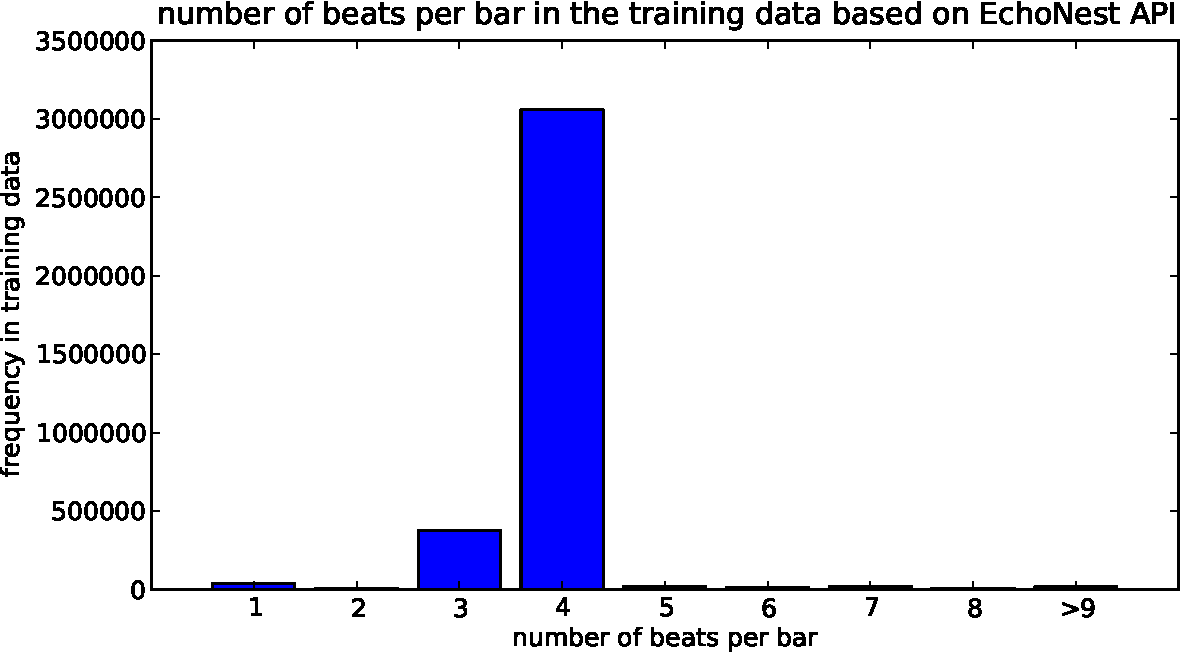
\includegraphics[width=.9\columnwidth]{bar_size_freq}
\end{center}
\caption{\small{
Frequency of the different bar size in the training data.
}}
\label{fig:barsize}
\end{figure}

Note that we do not claim that any of these informations (segments, beats, bars)
are perfectly accurate (\eg in \cite{Barrington2009a} authors obtain a better
song segmentation than Echonest). Practise showed us that they are reasonable, 
and the size of the data set should make up for the imperfections or noise.
We also believe that patches sizes based on a number of beats or bars are more
meaningful than an arbitrary time length. More on this in the experiments
(Subsection \ref{ssec:segment}).

\begin{figure}[htb]
\begin{center}
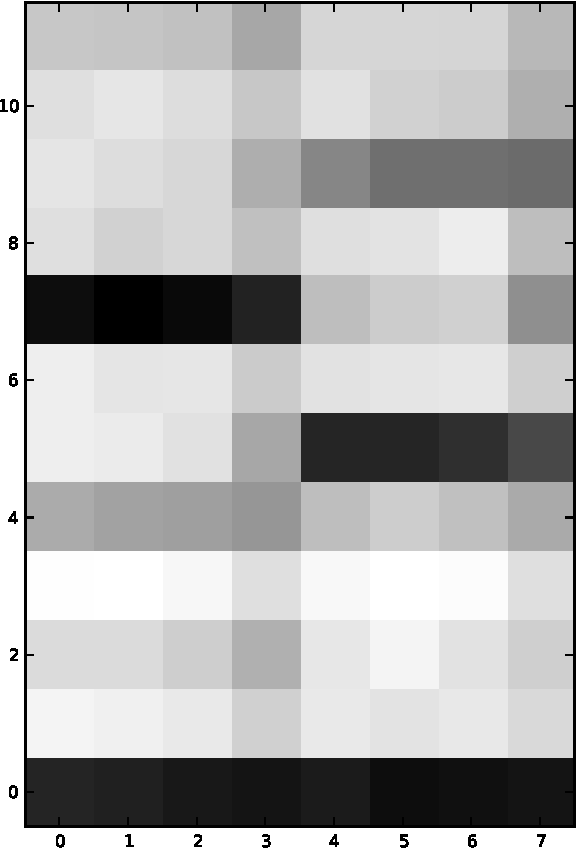
\includegraphics[width=.6\columnwidth]{code}
\end{center}
\caption{\small{A typical codeword from a codebook of size $200$. 
Patterns represented
$2$ bars and the pattern length was set to $8$.
}}
\label{fig:code}
\end{figure}


%\section{Algorithm}\label{sec:algo}
In this section we present the creation of the harmonic patterns from
the Echo Nest data.  Then we explain the online vector quantization algorithm
used to learn a codebook of those patterns.

%\subsection{Harmonic Patterns}
\subsection{Beat-Chroma Patches}
% Patterns are defined as a number of beats or bars. In the case of beats,
% we simply cut the set of chromas per beat every $N$ beats. In the case
% of bars, we gather all beats corresponding to the $N$ bars requested.
% The number of chroma vectors we get can vary. We resize the features in the
% time axis to a fixed length. Resizing over clipping can be argued over, 
% but it should
% preserve the main bar characteristics (such as a strong beat at the beginning
% or a note change in the middle).

We use the bar segmentation obtained from the analysis described in
the previous section to break a song into a collection of beat-chroma
``patches'', typically one or two bars in length. 
%
Because the bar length varies, depending on the meter of a particular
song (see Figure \ref{fig:barsize}), we resample each patch to a fixed
length of typically 4 to 8 beats.
% although the majority of the data contains bars that are 4 beats long

Finally, we normalize the patches with respect to the key by rotating
the pattern matrix so that the first row contains the most
energy. This can easily be seen in Figure \ref{fig:code}.
% We considered the same technique for rolling along the other axis and
% be invariant regarding the downbeat. However, it seems less robust to
% noise.
Each patch within a song is normalized independently, so exact
reconstruction of the original song requires knowledge of the
rotation index (key) for each patch.

The representation resulting from this process is invariant to both
the key and meter of the original song.  This enables the study of
broad harmonic patterns found throughout the data, without regard for
the specific musical context.
%
% In the context of clustering, this enables us to study harmonic
% pattern usage without maintaining clusters for the specific context a
% particular patterns occurs in,
In the context of clustering this avoids \eg obtaining separate
clusters for every major triad in duple or triple meter.
% Also, this implies that the pitch envelope is important rather than
% the actual pitches.
Something about why we're not interested in specific chords?

\subsection{Clustering}

We use an online version of the vector quantization algorithm
\cite{Gersho1991}, to cluster the beat-chroma patches described in the
previous section.
% This can also be seen as an online K-means.
For each sample from the data, the algorithm finds the closest cluster
in the codebook and updates the cluster centroid (codeword) to be
closer to the sample based on some learning rate $l$.
The clusters are updated as each data point is seen, as opposed to
once per iteration in the standard k-means algorithm.
The details are explained in Algorithm \ref{algo:vq}.
%
As in standard k-means clustering, the codebook is initialized by
choosing $K$ random points from our dataset.
%
Note that this algorithm, although not optimal, scales linearly with
the number of patches seen and can be interrupted at any time
while still resulting in an updated codebook. %not that this is important...
% The setting of the learning rate might become trickier, but this is
% not fundamentally a problem.

\begin{algorithm}
%\caption{Pseudocode of Vector Quantization}
\begin{algorithmic}
\STATE$l$ learning rate
\STATE$\{P_n\}$ set of patches
\STATE$\{C_k\}$ codebook of $K$ codes
%\STATE $m \leftarrow b$
\REQUIRE $0 < l \leq 1$
\FOR{$nIters$}
\FOR{$p \in \{P_n\}$}
\STATE$c \leftarrow min_{c \in C_k} dist(p,c)$
\STATE$c \leftarrow c + (p - c) * l$
\ENDFOR
\ENDFOR
\RETURN $\{C_k\}$
\caption{\small{Pseudocode of Online Vector Quantization. Note that we can 
replace the number of iterations by a threshold on the distortion over some 
test set.}
\label{algo:vq}}
\end{algorithmic}
\end{algorithm}



\section{Experiments}\label{sec:experiments}
In this section we present different clustering experiments. We introduce
our training data and our main testing data. Some detailed settings
of our algorithm are also provided. Then, we answer some common questions
about any clustering algorithms, for instance 
``how the number of codes affect the distortion''
and ``how many learning samples should we use''.
Note that we will present two additional experiments in 
Section \ref{sec:exps2}.


\subsection{Training: Cowbell Dataset}\label{sec:traindata}
We have $43,300$ tracks that were uploaded
to morecowbell.dj\footnote{http://www.morecowbell.dj/}, 
an online service that uses the Echo
Nest to produce a remixed version of
an uploaded music file that adds cowbell and other sound
effects in time with the music.
The $43.3$K songs, giving $\mathbf{3.7}$\textbf{M}
non silent bars, a bar usually
contains $4$ beats (Figure \ref{fig:barsize}).



\subsection{Testing: USPOP}\label{sec:testdata}
We had access to a low quality (32kbps) version of the songs in the uspop 2002 
data set \cite{uspop2002}.
This well-known data show a great diversity of pop songs, but is not particular
otherwise\footnote{We 
also tried to use Tzanetakis dataset, 
%\cite{Tzanetakis2002a},
but the $30$ seconds segments seemed hard to analyze by the Echo Nest API, 
most did not contain any bar.}.
uspop2002 serves as testing set to measure how well a codebook learned on
the Cowbell data set can represent new songs. We get Echo Nest features
for $8651$ songs of that dataset.


\subsection{Setting}\label{ssec:setting}
We take one or two bars and normalize the patches to size 4 or 8 respectively.
We roll the patch to be invariant to the key (on the patch level, not on
the song level). We learn a codebook of size $K$ over the cowbell dataset 
using the VQ algorithm (Algorithm \ref{algo:vq}). A typical learning rate 
is $0.01$ for $200$ iterations over the whole dataset.

We use the codebook to encode our testing set (see Section \ref{sec:testdata}).
Each pattern is encoded with only one code. We can measure the average
distance between a pattern and its encoding. We can also measure the use
of the different codes, \ie the size of the cluster around a code.

As a distance measure (or distortion measure) between patterns, we use
the average squared euclidean distance. In details, if a pattern $p1$
is composed of elements $p1_{i,j}$, and similarly for a pattern $p2$,
the distance between $p1$ and $p2$ is:
\begin{eqnarray}
  dist(p1,p2) = \sum_{i,j} (p1_{i,j} - p2_{i,j})^2 / size(p1)  \label{eq:dist}
\end{eqnarray}
We assume $p1$ and $p2$ have the same size.


\subsection{Basic Properties}
This section present some fundamental results of the clustering algorithm.
These are important, but do not change the larger picture. Due to space
constraints, we give few details and refer to the figures.
\begin{itemize}
\item A larger dataset gives a better encoding codebook. See Figure
\ref{fig:data_sizes}.
\item A larger codebook better encodes new songs. See 
Table \ref{tab:cbsize}.
\item Larger patterns are more difficult to encode, thus require
larger codebooks. See Figure \ref{fig:perbeat}.
\end{itemize}

These properties are important to verify and for reproducing the experiments, 
but they are not surprising for a clustering algorithm.

\begin{figure}[htb]
\begin{center}
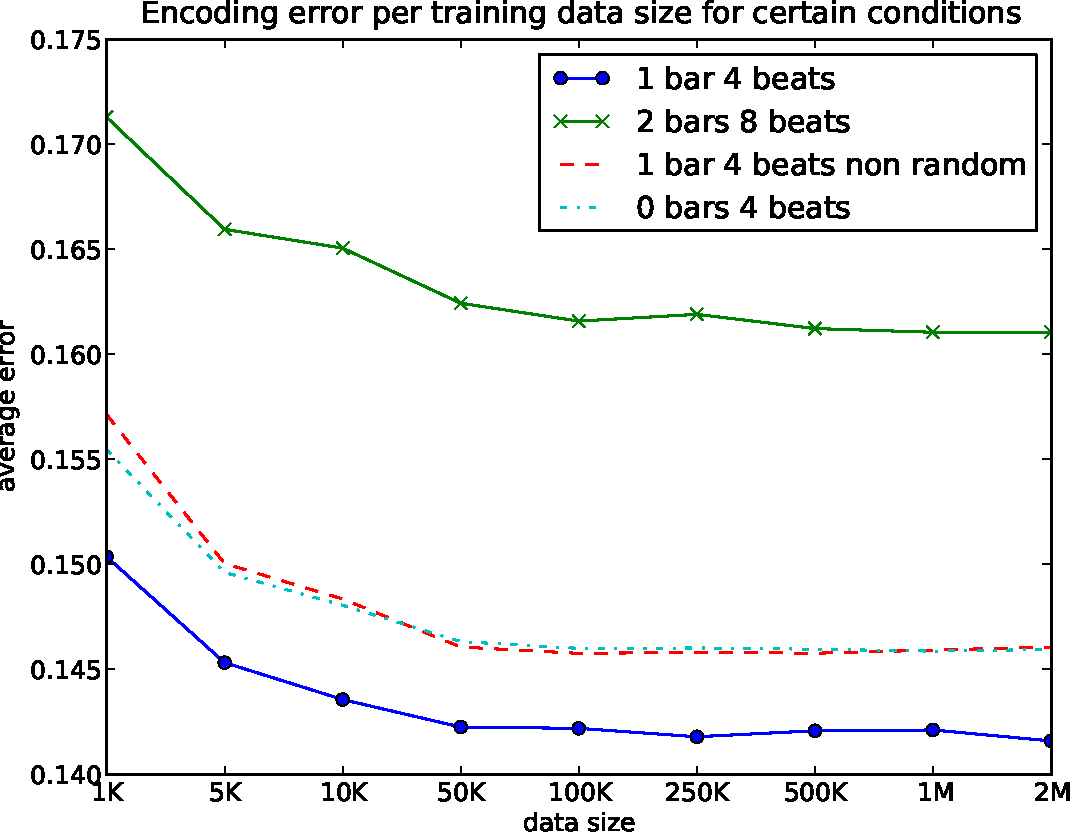
\includegraphics[width=.99\columnwidth]{data_sizes}
\end{center}
\caption{\small{Distortion for a codebook of size $100$ encoding one bar
at a time, a bar being represented by $4$ chroma feature vector.
Therefore, a codeword or a pattern is of size $12$ x $4$ = $48$.
Distortion measure on the test data set. Data size tested range
from $0$ (just initialization) to $500$ thousand. Patterns were selected at
random from the dataset of approximately $3,7$ million patterns, except
for the dotted line (non random in the legend). In that case we took the
first $N$ samples in our dataset. The difference is only visible for small
training sets ($1$K).
}}
\label{fig:data_sizes}
\end{figure}

\begin{table}
\begin{center}
\begin{tabular}{|l|l|c|}
\hline
\# codes & distortion \\ \hline \hline
1 & $0.066081$ \\
10 & $0.045579$ \\
50 & $0.038302$ \\
100 & $0.035904$ \\
500 & $0.030841$ \\ \hline
\end{tabular}
\end{center}
\caption{\small{Experiment with the codebook size. We train on patterns
corresponding to $1$ bar resized to $4$ beats. 
The number of training samples is $50000$.
}}
\label{tab:cbsize}
\end{table}


\begin{figure}[htb]
\begin{center}
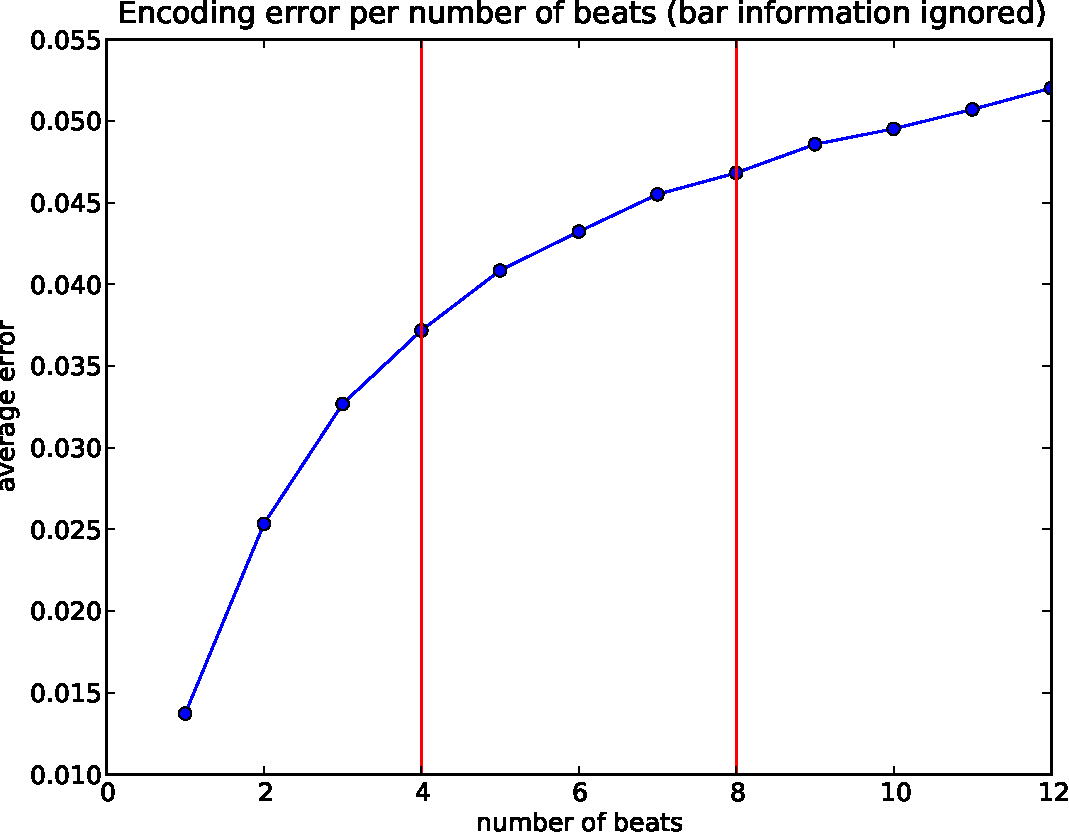
\includegraphics[width=.9\columnwidth]{encoding_per_beat}
\end{center}
\caption{\small{Encoding larger and larger patterns with a fixed size
codebook. The size of the pattern is defined by the number of beats,
the bar information was not taken into account for that experiment.
}}
\label{fig:perbeat}
\end{figure}


% REMOVING THE FOLLOWING SUBSECTION ON RATE - DISTORTION
\iffalse
\subsection{Music Randomness}\label{ssec:random}
It will not surprise any reader, music is not random. This fact should
become apparent in our experiments in the following way. Information
theory tells us that if the signal to encode doubles, we need to square
the size of the codebook to encode it with the same distortion.

To help the intuition, here is an example. Imagine a binary array of 
length $1$. We need two
codes to encode perfectly: $(0)$ and $(1)$. If the binary array is now of
length $2$, we now need four codes: $(0,0)$, $(0,1)$, $(1,1)$ and $(1,0)$.

Since music is not random, we expect that squaring the codebook when the
pattern size doubles will rather give improved results than constant ones.
See Figure \ref{fig:size_pattern}.

% see generate_expo_codes_curves.py to generate the following figure:
\begin{figure}[htb]
\begin{center}
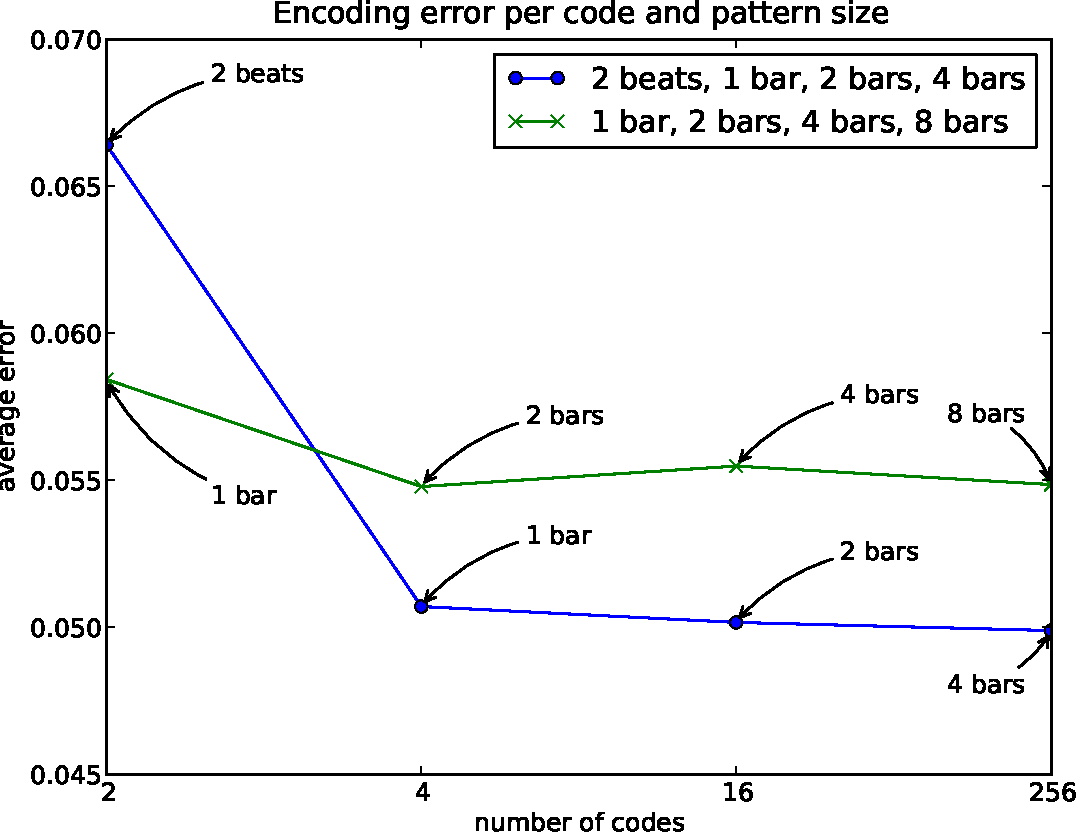
\includegraphics[width=.99\columnwidth]{codesize_patternsize}
\end{center}
\caption{\small{
Experiment on squaring the codebook size when the pattern size doubles.
Each line represent $4$ codebook sizes: $2$, $4$, $16$ and $256$.
The pattern size range from $1$ for $1/4$ of a bar to $32$ for $8$ bars.
If everything was random, each of these lines should be flat. The training
size was fixed to $128$K samples.
}}
\label{fig:size_pattern}
\end{figure}
\fi


\section{Visualization} \label{sec:visu}
% The goal here is to give an intuition to the reader of what kind of
% typical patterns do we get. We also want to have a feel for what the
% clusters look like, how many boring sustained notes are encoded in the
% codebook, can the codebook describes the complexity of the music space, etc.


\subsection{Codebook}\label{sec:codebook}

We train a codebook of size $200$ over patterns of size $12$x$8$ covering
$2$ bars at a time. Results shown are on a second testing set, see
Subsection \ref{ssec:artist}.


The 25 most frequently used codewords in the test set are shown in
Figure \ref{fig:codes1}.  
The frequency of use of these codewords are shown in Figure \ref{fig:freqs}.
The codewords primarily consist of sustained
notes and simple chords.  Since they are designed to be key-invariant,
specific notes do not appear.  Instead the first 7 codewords
correspond to a single note sustained across two bars (codeword 1),
perfect fifth (codes 2 and 3) and fourth intervals (codes 4 7), and a
major and minor triads (codeword 6 and 5).  Many of the remaining
codewords correspond to common transitions from one chord to another,
\eg a transition from one major triad to another (\ie Cmaj
$\rightarrow$ Fmaj assuming that chroma 0 is C) in codes 8 and 10 and
the reverse transition in code (\ie Fmaj $\rightarrow$ Cmaj) in code
22.  Does this transition have a better name like ``relative x''?

\begin{figure}[h]
\begin{center}
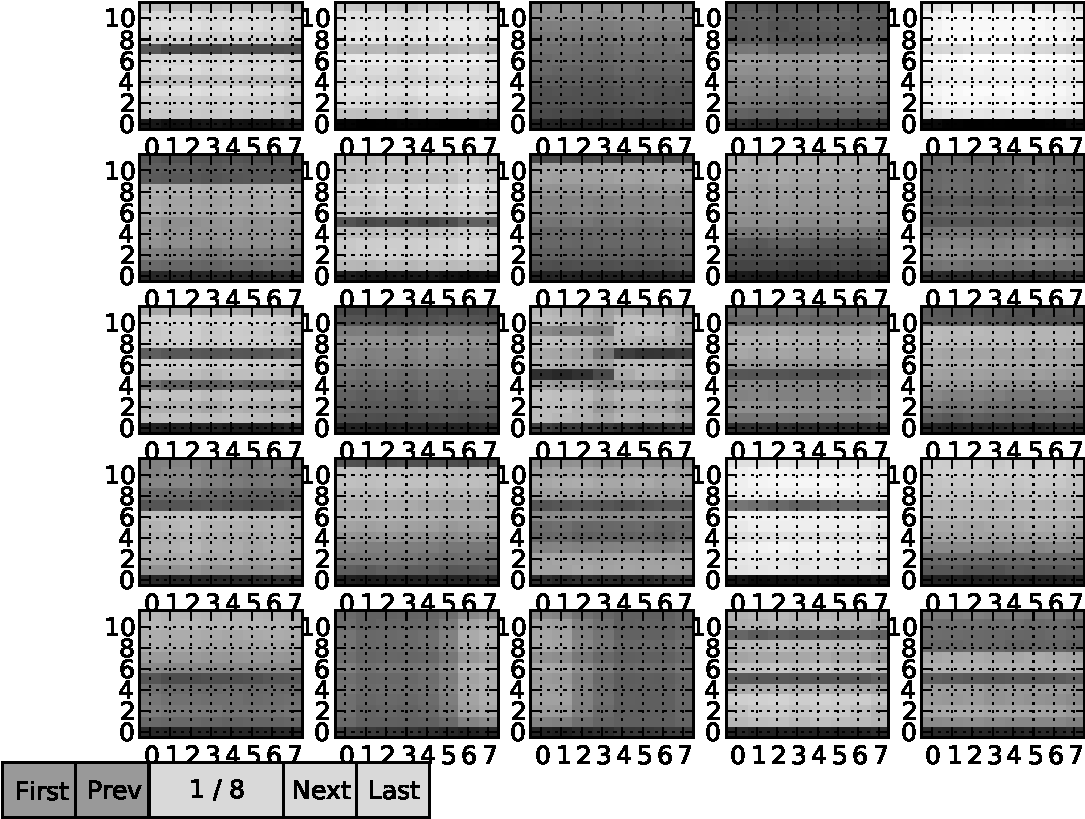
\includegraphics[width=.9\columnwidth]{codes1}
\end{center}
\caption{\small{
Most used codes in the codebook in term of frequency of use in the test
set (artist20, see Subsection \ref{ssec:artist}). 
This codebook was of size $200$ and trained on $2$ bars, pattern
size is $12$x$8$. Code in Figure \ref{fig:code} is the $8$th most used
here (second row, third column). 
Numbers display are the index (from most used to least) and in parentheses
the percentage of use in the whole collection times.
There is $71832$ patterns in total in the dataset.
}}
\label{fig:codes1}
\end{figure}

\begin{figure}[htb]
\begin{center}
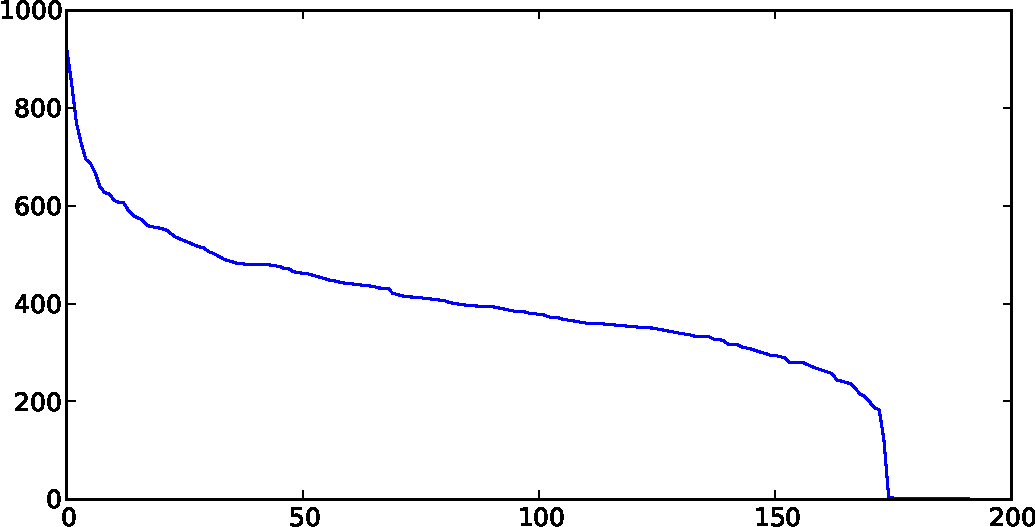
\includegraphics[width=.7\columnwidth]{freqs}
\end{center}
\caption{\small{
Frequency of use of the patterns in Figure \ref{fig:codes1} on the
artist20 dataset. 
There is $71832$ patterns in total in the dataset.
Note that all codes were initialized with a random
sample from the training set, some might not just be present in this
test set.
}}
\label{fig:freqs}
\end{figure}

Another interesting visualization uses LLE\footnote{implementation:
  \url{http://www.astro.washington.edu/users/vanderplas/coding/LLE/}}
algorithm \cite{Roweis2000} to display codewords arranged in
coherent groups. See Figure \ref{fig:lle}.

Finally, more related to our particular data, we try to assess how many
sustained patterns are represented in the codebook. We look at
the average variance over time in Figure \ref{fig:code_var}.
25\% of the codebook correspond
to very simple sustained patterns similar to the top row of Figure
\ref{fig:codes1}. For $2$ bars codewords, it seems that interesting
patterns appear in only $33$\% of the data.

Showing codewords of $2$ bars is practical and consistent with our experiments
in Section \ref{sec:exps2}. However, longer codewors can also reveal
interesting structures. A random samples of such codewords is presented
in Figure \ref{fig:codes8bars}


\begin{figure}[htb]
\begin{center}
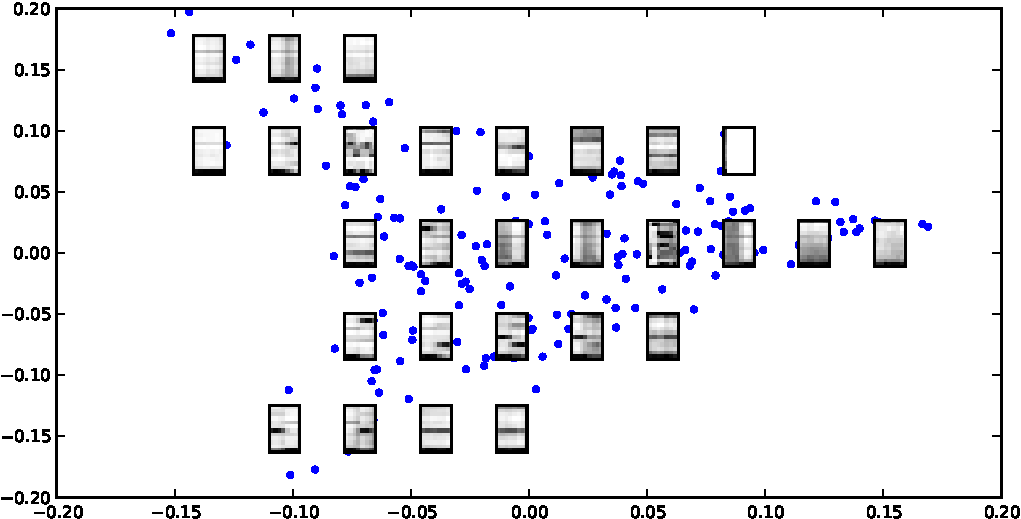
\includegraphics[width=.9\columnwidth]{codes_lle}
\end{center}
\caption{\small{
Locally linear embedding (LLE) visualization of the codebook.
LLE tries to keep near neighbors (here according to euclidean distance)
in the same $2$D neighborhood. Shown patterns were randomly selected
in each neighborhood.
}
ronw: I think this figure would be better if it only included the
bottom subplot.
}
\label{fig:lle}
\end{figure}

\begin{figure}[htb]
\begin{center}
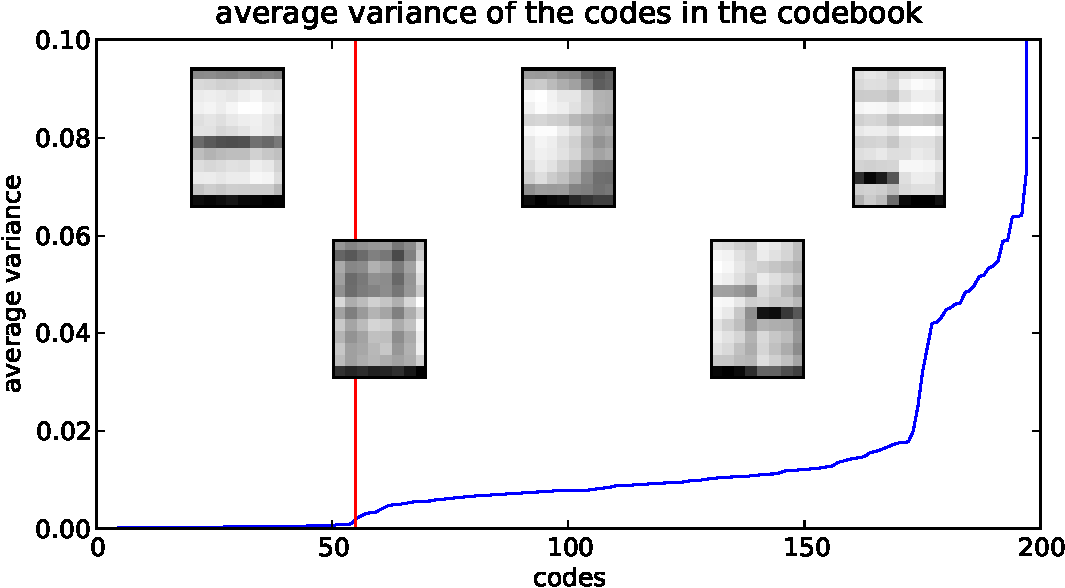
\includegraphics[width=.9\columnwidth]{code_variance}
\end{center}
\caption{\small{Average variance in time of a codebook. The vertical
axis cuts at the $63$rd pattern, a rough estimate of the number of 
sustained note patterns.
}}
\label{fig:code_var}
\end{figure}

\subsection{Cluster}
Once we understand the kind of codebook we create, we naturally want
to visualize the clusters, \ie the patterns from actual song that
surround a given centroid. Unsurprisingly, real patterns tend to be
noisier than codes. However, centroids seem to capture important aspects
of the patterns. We could compare the centroids with the result of
a lowpass filtering. In Figure \ref{fig:cluster} we show elements of the same
cluster, and in Figure \ref{fig:cluster_diff}, we emphasize the difference
with the centroid.

\begin{figure}[htb]
\begin{center}
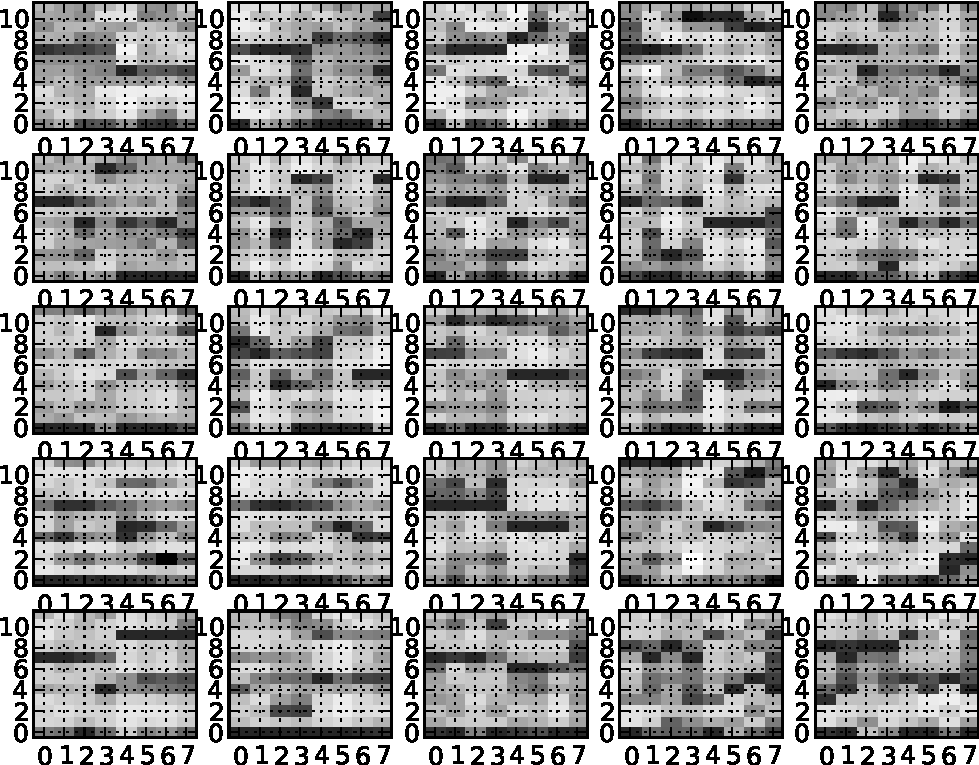
\includegraphics[width=.9\columnwidth]{close_patterns1}
\end{center}
\caption{\small{Cluster around centroid presented in
Figure \ref{fig:code}. Taken from the artist20 dataset, the cluster
size is actually $639$. Shown samples were randomly selected.
}}
\label{fig:cluster}
\end{figure}

\begin{figure}[htb]
\begin{center}
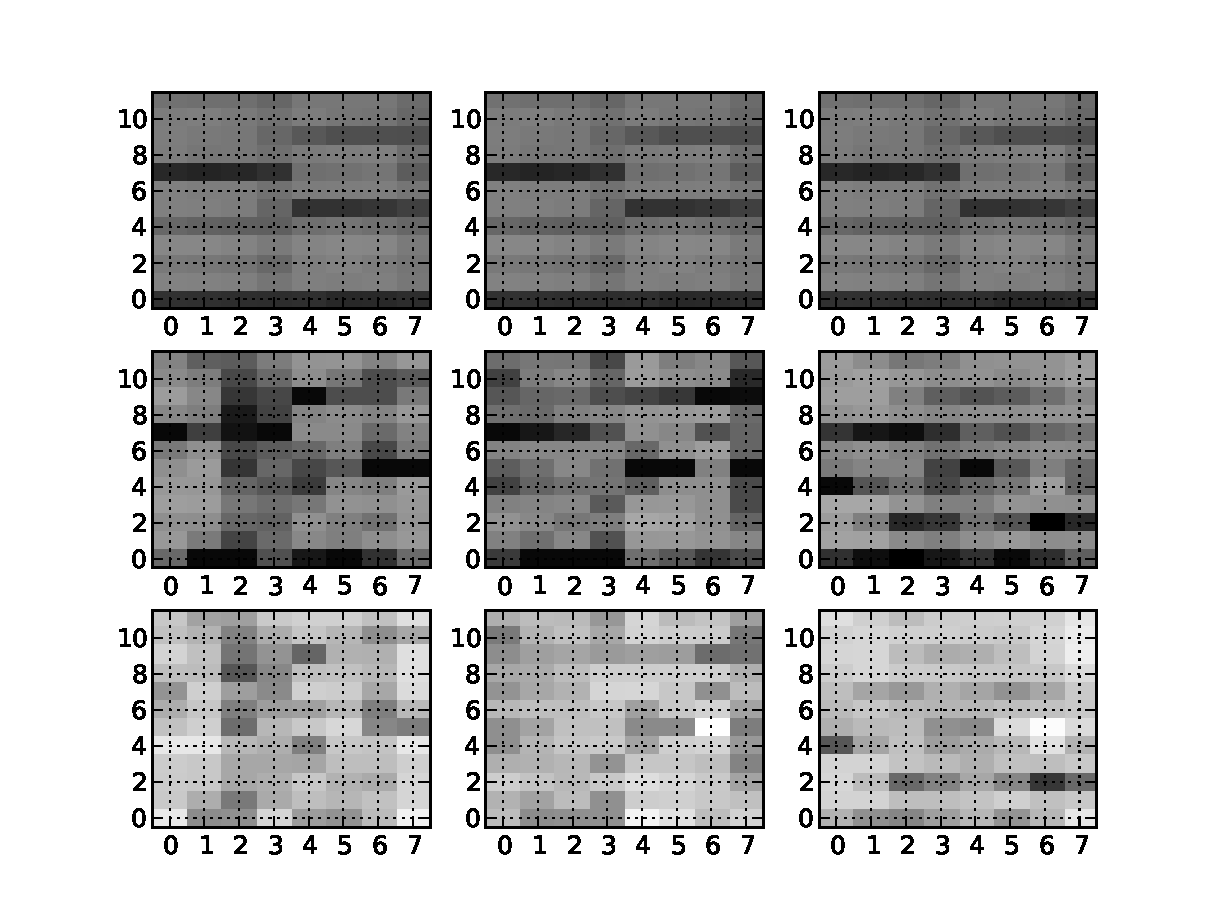
\includegraphics[width=.8\columnwidth]{close_patterns_diff}
\end{center}
\caption{\small{First three patterns of figure \ref{fig:cluster}
($2$nd line) presented with the centroid from Figure \ref{fig:code}
($1$st line) and the absolute difference between both ($3$rd line).
}
ronw: does this figure really add all that much?
}
\label{fig:cluster_diff}
\end{figure}

\begin{figure}[htb]
\begin{center}
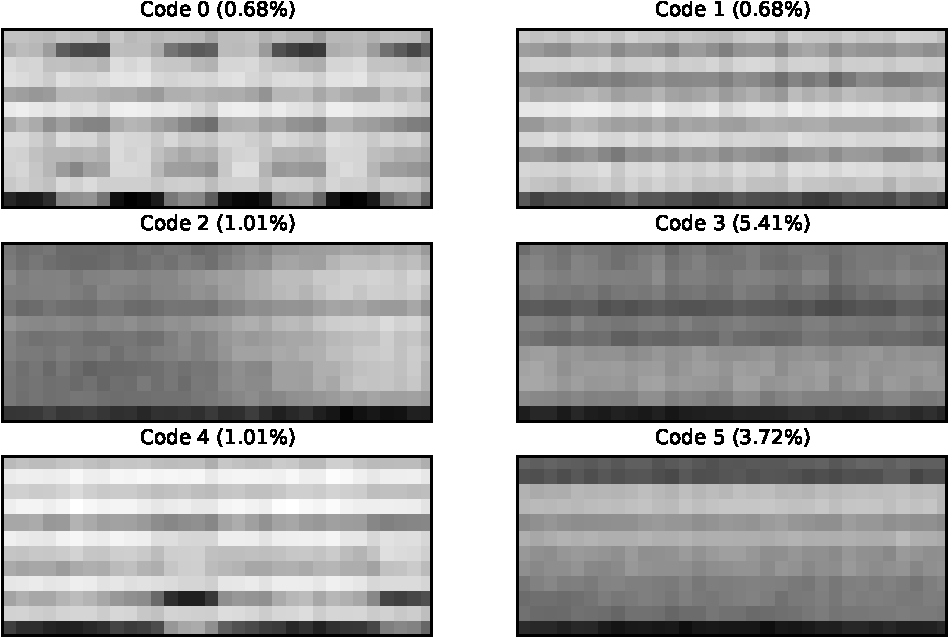
\includegraphics[width=.8\columnwidth]{codes_8bars}
\end{center}
\caption{\small{Sample of longer codewords spanning over $8$ bars. Codewords
selected randomly from a codebook of size $200$. As usual, we see sustained
notes, but also some long-term structures.
}}
\label{fig:codes8bars}
\end{figure}


\subsection{Example song encoding}

Figure \ref{fig:encodesong} shows a typical example of encoding a song
using the codebook described in Section \ref{sec:codebook}.  Both the
Echo Nest chroma features for an example song and the corresponding
quantization are displayed.  The quantized representation retains
dominant harmonic structure of the original features, but is smoothed
in time due to the use of 2 bar long codewords.
%
This is consistent with the codebook described in Section
\ref{sec:codebook} which primarily consists of sustained chords across
4 or 8 beats.

\begin{figure}[htb]
\begin{center}
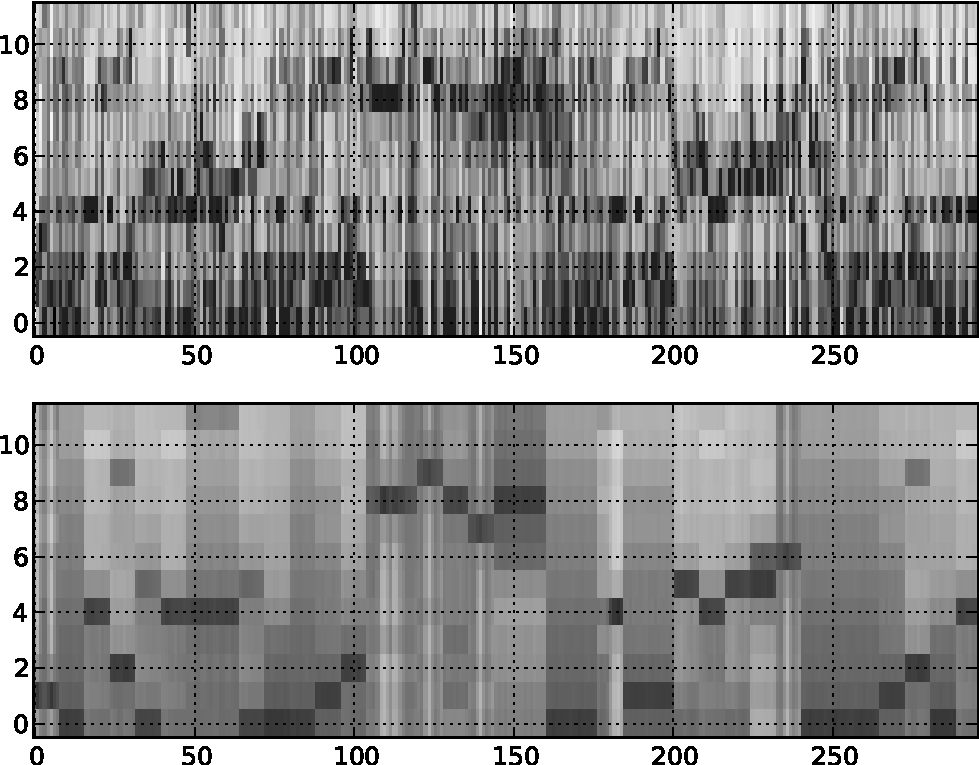
\includegraphics[width=.9\columnwidth]{song_encoded}
\end{center}
\caption{\small{Good Day Sunshine by \textit{The Beatles}.
Original song and its encoding using a $200$ codes codebook learning
$2$ bars at a time.
}}
\label{fig:encodesong}
\end{figure}


\section{Applications}\label{sec:exps2}
We have shown the basic properties of our clustering algorithm in
Section \ref{sec:experiments}. In Section \ref{sec:visu}, we showed
how to visualize the codebook and the clusters. We know move on to
show other applications that can take advantage of our clustering.
In the next two subsections, we talk about song segmentation and
artist recognition. Our algorithm was not devised for any of these tasks,
but some information contained in the centroids can be naturally used.

\subsection{Song Segmentation} \label{ssec:segment}
We explained that we used bars as defined by the EchoNest algorithm to
train our patterns. Let's assume once again that those bars are
reasonable. We investigate whether we could recover the bar segmentation
of new songs from our codebook. It would helps us assert that codes
encodes something related to bars, for instance a strong beat at the
beginning. Results are shown \ref{tab:offset}. We find the right segment
with an accuracy of $62\%$ where random is $25\%$. Details of the
experiment follow.

We train a codebook of size $100$ on bars resized to $4$ beats. Then,
we take the longest sequence of bars of $4$ beats in the test set.
As we mentioned before, $4$ beats is the most common (by far!) bar size
in terms of beats according to the EchoNest API. We then encode this
sequence using an offset of $0$, $1$, $2$ or $3$ beats. The best offset
is the one that gives the encoding with the lowest distortion. The
good answer is an offset of $0$.

The result presented here suggest a dynamic programming setting where
we could find the optimal bar segmentation according to our codebook. 
We could try
all possible bar length (in terms of beats) and not restrict ourselves
to $4$ beats bars and offsets between $0$ and $3$. This is part of
our future work.

\begin{table}
\begin{center}
\begin{tabular}{c|c}
%\hline
offset & \% of times chosen \\ \hline
0 & $\mathbf{62.6}$\\
1 & $16.5$\\
2 & $09.4$\\
3 & $11.5$\\
\end{tabular}
\end{center}
\caption{\small{
Best offset according to our codebook. The real one is $0$.
Random guess gives an accuracy of $25$\%.
}}
\label{tab:offset}
\end{table}

\subsection{Artist Recognition} \label{ssec:artist}

We apply our codebook to the artist recognition task.
Our data set encompass $1402$ songs from $20$ artists, 
mostly rock and pop of different subgenres. Results exist in the
litterature for that set \cite{Ellis2007}. The best accuracy is
$59\%$, whereas using only chroma as a representation yields an
accuracy of $33\%$. The latter results is obtained through a
gaussian mixture model.

Once again, the clustering method proposed in this work is not
intended to perform well at artist recognition. An obvious fact is that
we lose all timbral information which would be useful. However, we can
imagine that some artist use more often some patterns than others.
Our accuracy result is $23.4\%$ while random
is around $5\%$. 
The confusion matrix can be seen in Figure \ref{fig:conf_mat}.
Details of the experiment follow.

All songs in the artist dataset are encoded as an histogram of the codes
used in that song. The frequency values are normalized by the number
of patterns in the song. We test each song in a leave-one-out setting.
Leaving aside the test song, we represent each of the $20$ artists by the 
average of
the song histograms of that artist. The test song is compared to
the histogram of each artist using euclidean distance.


\begin{figure}[htb]
%\begin{center}
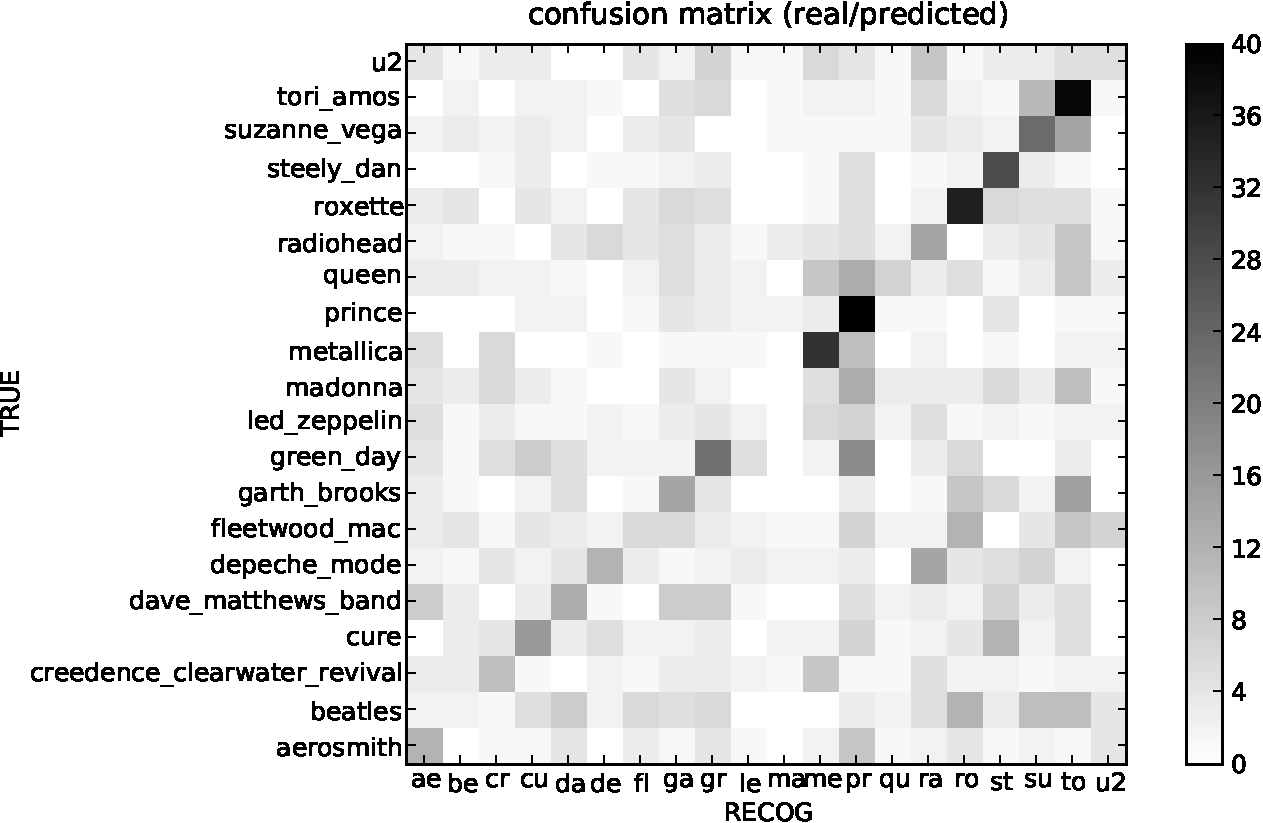
\includegraphics[width=.9\columnwidth]{conf_mat_per_artist}
%\end{center}
\caption{\small{Confusion matrix for artist recognition task.}}
\label{fig:conf_mat}
\end{figure}

Looking at the most typical patterns per artist can be insightful.
To find these patterns, we compare its use by one artist and divide
by its use by all artists. In Figure \ref{fig:typicalpat} we see 
Metallica's pattern, then Tori Amos and
Suzanne Vega's pattern. These three artists were easily identified.

Artists like metallica are characterized by ``wideband'' patterns -
featured muddled due to noisy acoustics - lots of transients,
distortion, etc.  (not by cleaned up by EN's feature analysis)

% ignoring the two following figures
\iffalse
\begin{figure}[htb]
\begin{center}
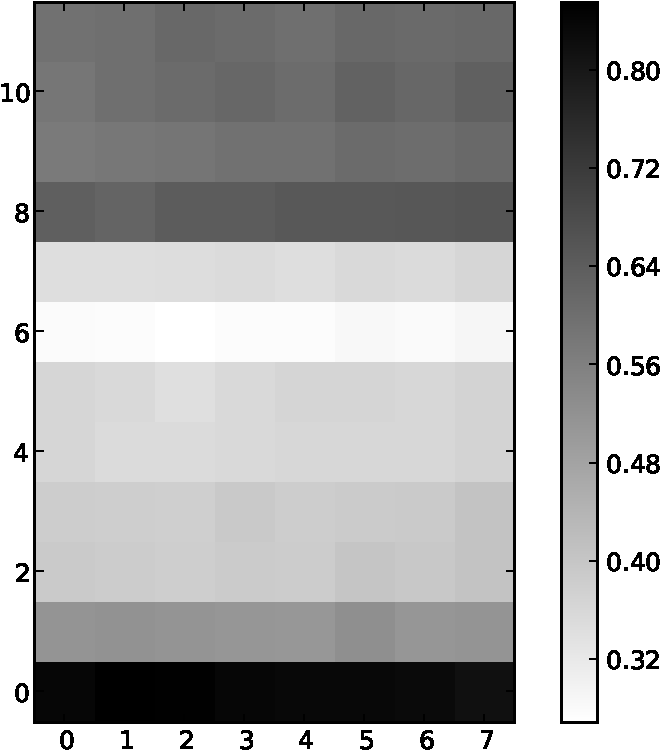
\includegraphics[width=.4\columnwidth]{metallica_pattern}
\end{center}
\caption{\small{Most typical pattern for Metallica.
COULD BE MIXED WITH TORI AMOS FIGURE.
}}
\label{fig:metallica}
\end{figure}

\begin{figure}[htb]
\begin{center}
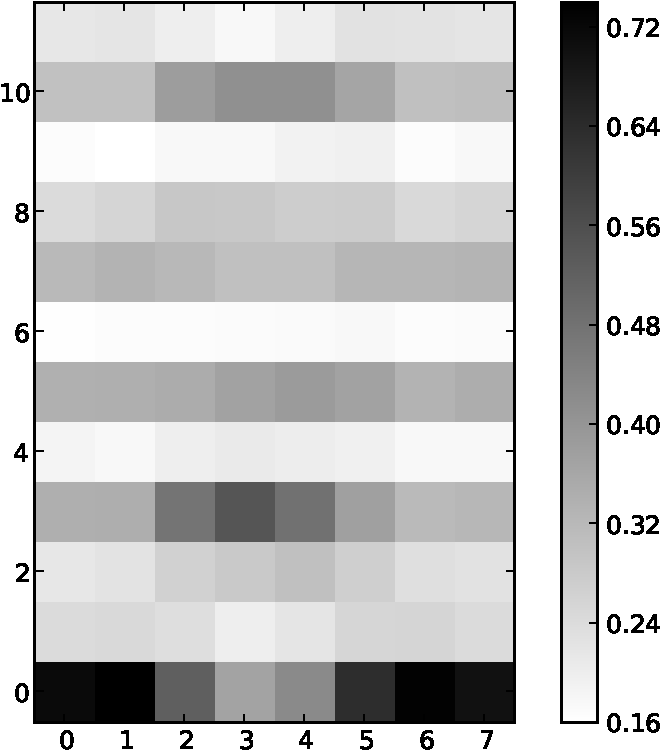
\includegraphics[width=.4\columnwidth]{toriamos_suzannevega_pattern}
\end{center}
\caption{\small{Most typical pattern for Tori Amos and Suzanne Vega.
    Can we show the top 2 or 4 for each to get a better idea?}}
\label{fig:amosvega}
\end{figure}
\fi


\begin{figure}[htb]
  \centering
  \subfloat[][\small{Metallica}]{\label{fig:metallica2}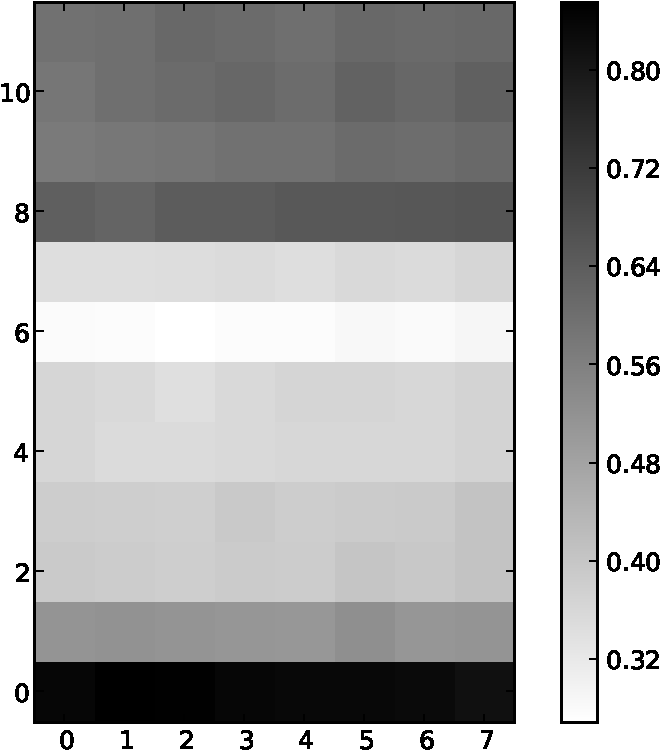
\includegraphics[width=0.35\columnwidth]{metallica_pattern}}
  \hspace{5mm}                
  \subfloat[][\small{Tori Amos / Suzanne Vega}]{\label{fig:amosvega2}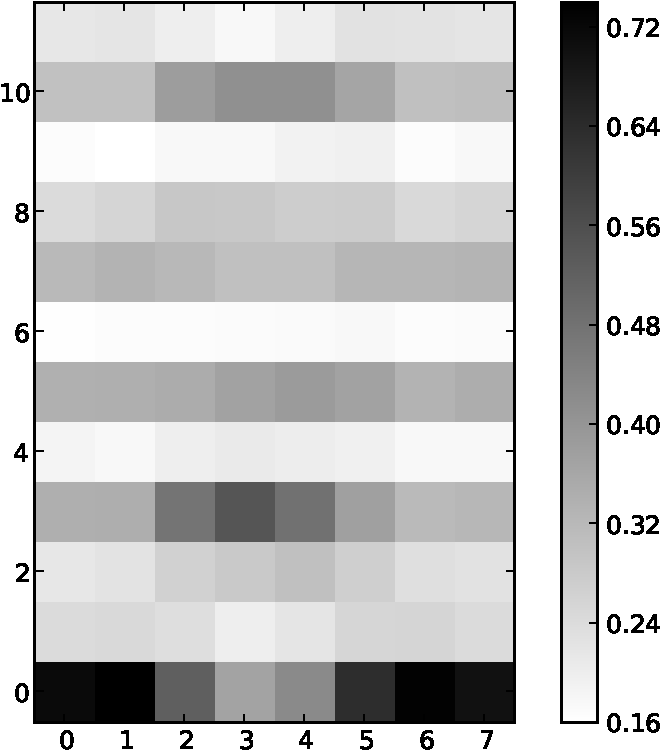
\includegraphics[width=0.35\columnwidth]{toriamos_suzannevega_pattern}}
  \caption{\small{Typical patterns for different artists.}}
  \label{fig:typicalpat}
\end{figure}



\section{Conclusion and Future Work}
We presented a practical method to perform large-scale clustering of
harmonic patterns. We assessed the basic properties of the method through
experiments on a large collection of music. We suggested many ways
to interpret the data (such as LLE) and assert the merit of the codebook
through further experiments.
We discussed the possibility to move to even larger scales
and we provided our source code\footnote{Code not yet released to preserve
submission's anonymity}.

As for enhancements, we specifically did not compress our features using
gaussian mixtures or other generative model. That being said, these methods
could be use to develop better distance measures between patterns.
The use of the euclidean distance is arbitrary. Summarizing patches
with gaussians, and then comparing the distance between those gaussians,
could reduce the influence of the noise in the distance measure.

Moving on to larger scales, we could imagine merging codes together and
splitting some on two if the clusters become too small or too large.We could
also cluster the codebook itself, in a similar fashion as hierarchical
gaussian mixtures \cite{Vasconcelos2001}.
%  (similar idea used for indexing \cite{Muja2009})


\small
%\section{Acknowledgements}
%Thierry is NSERC graduate fellow, or some title like that.
%Ron has a grant too.
% Graham for the NMF stuff and numerous discussions.

%\begin{thebibliography}{citations}
%\bibitem{Someone:04} 
%X. Someone and Y. Someone:
%{\it Title of the Book},
%Editorial Acme, Utrecht, 2004.
%\end{thebibliography}

\bibliography{tbm_bib}





\end{document}
